\subsection{Architektur, Funktionsweise und Implementierung}
\label{sec:prototype_arch} 
    Da momentan weder eine Standardisierung noch Best Practices von Blockchainarchitekturen existieren, wurde die Architektur des Prototypen anhand der Dokumentation des Frameworks\cite{ComposerDocs}, sowie den darin enthaltenen Beispielen ausgearbeitet. 
    Sollte eine Beschreibung direkt auf einen der beiden Anfoderungskataloge, die in \fref{sec:prototype_func_req} und in \fref{sec:prototype_sec} gesammelt wurden beziehen, so wird diese mit der entsprechenden Referenz verdeutlicht.
    
    \subsubsection{Konzept}
        Das Blockchain-Netzwerk für den Prototypen umfasst ein oder mehrere Herstellerserver, ein oder mehrere Schlösser, sowie ein oder mehrere Nutzer und basiert auf einer private/permissioined Blockchain. 
        Sollten Alice und Bob je ein Schloss vom gleichen Hersteller haben, aber nicht im gleichen ,,Haus`` wohnen, so entstehen zwei unterschiedliche Blockchain-Netzwerke, die jeweils voneinander isoliert sind.
        \smallskip\\
        \noindent Im Modell des Prototypen gibt es demnach drei verschiedene Teilnehmertypen, wobei für ein minimales funktionales Netzwerk mindestens Teilnehmer jedes Typs vertreten sein muss. 
        In dem Netzwerk kann jeder Teilnehmer mit allen anderen Teilnehmern kommunizieren.
        \begin{enumerate}[noitemsep]
            \item \textbf{Hersteller/Vendor}: Zur Initialisierung, Zurücksetzung, Updates, \dots
            \item \textbf{Schloss/Lock}: das physische Schloss, welches bei einem Nutzer installiert wird
            \item \textbf{Nutzer/User}: öffnet/schließt ein oder mehrere Schlösser, verwaltet u.U. andere Nutzer
        \end{enumerate}
        
        \noindent In \fref{fig:pt_network} ist ein Beispiel mit zwei verschiedenen Herstellern \colorbox{light-gray}{\lstinline{V1,V2}}, drei Schlössern \colorbox{light-gray}{\lstinline{L1,L2,L3}} und drei Nutzern \colorbox{light-gray}{\lstinline{U1,U2}}. 
        Insgesamt wurden vier Schlüssel \colorbox{light-gray}{\lstinline{K1-K4}} ausgestellt.
        \colorbox{light-gray}{\lstinline{L1}} und \colorbox{light-gray}{\lstinline{L2}} sind von Hersteller \colorbox{light-gray}{\lstinline{V1}}, \colorbox{light-gray}{\lstinline{L3}} stammt von Hersteller \colorbox{light-gray}{\lstinline{H2}}. 
        \colorbox{light-gray}{\lstinline{U1}} hat mit den beiden Schlüsseln \colorbox{light-gray}{\lstinline{K1,K2}} die Möglichkeit \colorbox{light-gray}{\lstinline{L1}} und \colorbox{light-gray}{\lstinline{L3}} zu öffnen. 
        Der Nutzer \colorbox{light-gray}{\lstinline{U2}} kann mit \colorbox{light-gray}{\lstinline{K3}} und \colorbox{light-gray}{\lstinline{K4}} die Schlösser \colorbox{light-gray}{\lstinline{L2}} und \colorbox{light-gray}{\lstinline{L3}} öffnen.
        \begin{figure}[H]
    		\centering
    		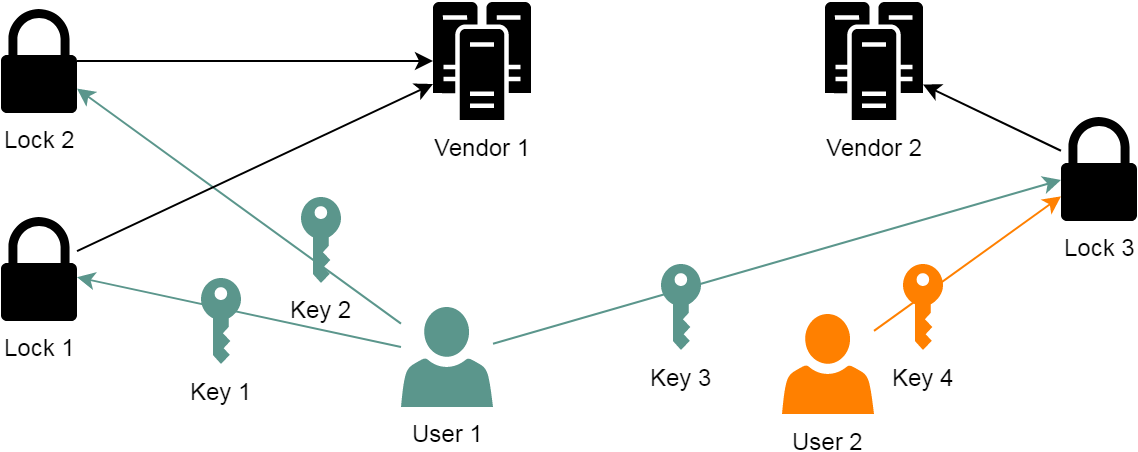
\includegraphics[width=\textwidth]{graphics/pt_network.png}
    		\caption[Beispiel eines von Beziehungen im Prototypen-Netzwerk]{Beispiel von Beziehungen eines Netzwerks, welches aus der Definition des Prototypen entstehen könnte}
    		\label{fig:pt_network}
    	\end{figure}
        \noindent Je nach Teilnehmertyp werden erlaubte Operationen innehalb des Netzwerkes mittels der \gls{acl} eingeschränkt. 
        Die Zugriffskontrolle für den Teilnehmertyp ,,Nutzer`` erfolgt zusätzlich auf einer feingranulareren Ebene über ein dafür angelegtes Attribut \colorbox{light-gray}{\lstinline{UserRole}} mit dem in \fref{tab:prototype_rbac} dargestellten Berechtigungskonzept. 
        Es ist rollenbasiert und ist wurde analog zu \fref{tab:rbac} entworfen. 
        Anders ist jedoch, dass angelehnt an öffentliche Netzwerke, alle Nutzer des Netzwerkes alle Informationen, die in dieser gespeichert wurden einsehen, aber nicht verändern können. 
        Wie in \fref{tab:prototype_rbac} verdeutlicht, gibt es die Rollen ,,Besitzer`` und ,,Gast`` mit unterschiedlichen Berechtigungen (\ref{fa:3}, \ref{fa:4}). 
        \begin{table}[H]
		    {\footnotesize
		    \centering
            \begin{tabular}{|m{0.14\textwidth}|m{0.14\textwidth}|m{0.14\textwidth}|m{0.14\textwidth}|m{0.14\textwidth}|m{0.14\textwidth}|}
                \hline
                \textbf{Rolle/Recht} &\textbf{Unlock}  & \textbf{Log einsehen}  & \textbf{Nutzer verwalten}  & \textbf{Rollen\-verwal\-tung} & \textbf{Schloss zurück\-setzen}  \\ \hline
                \textbf{Owner}       & \checkmark      & \checkmark             & \checkmark                 & \checkmark                    & \checkmark                       \\ \hline
                \textbf{Guest}       & \checkmark      & \checkmark             & ~                          & ~                             & ~                                \\ \hline
            \end{tabular}
            }
            \caption[Rollenbasierte Zugangskontrolle des Prototypen]{Rollenbasierte Zugangskontrolle des Prototypen. Ist ein Haken gesetzt, so wird der Rolle in der Spalte links das Recht aus der entsprechnenden Spalte gewährt.}
            \label{tab:prototype_rbac}
        \end{table}
        \noindent Schlüssel werden als Asset repräsentiert und von Nutzern verwendet, um ein Schloss zu öffnen(\ref{fa:2}). 
        Optional können die Schlüssel mit einem Ablaufzeitpunkt zeitlich eingeschränkt sein(\ref{fa:5}). 
        Es wird ein Schlüssel je Nutzer und Schloss ausgestellt. 
        Somit gäbe es beispielsweise bei zwei Schlössern \colorbox{light-gray}{\lstinline{L1,L2}} und einem Nutzer \colorbox{light-gray}{\lstinline{U1}} im Netzwerk zwei Schlüssel: \colorbox{light-gray}{\lstinline{U1arwL1,U1arwL2}}. \\
        Schlüssel sind nach Erstellung nicht modifizierbar und werden, falls ein Ablaufzeitpunkt angegeben wurde gelöscht. 
        Beim Öffnen des Schlosses geprüft, ob der öffende Nutzer das entsprechende Schlüsselasset besitzt und im Schloss eine Referenz auf den Schloss gespeichert. 
        Wird das Schloss wieder verriegelt, so wird die Referenz wieder gelöscht. 
        Hiermit kann einerseits sichergestellt werden, dass das Schloss geschlossen ist, wenn dieses keine Referenzen auf Schlüsselassets besitzt, andererseits wird jegliche Nutzung des Schlosses auf der Blockchain dokumentiert. 
        \medskip\\
        \noindent Mittels der in \fref{sec:prototype_composer} vorgestellten Mechanik des Historians werden nach diesem Konzept folgende Informationen also in der Blockchain gespeichert:
        \begin{itemize}[noitemsep]
            \item Erstellen, Modifizieren und Löschen von Ressourcen (Vendor, Lock, User, Key)
            \item Wann von wem welches Schloss geöffnet wurde und welchen Zustand dieses hat
            \item Welche Person welche Rolle inne hat und von wem diese gewährt wurde
            \item Jegliche erfolgreich abgeschlossenen Transaktionen
        \end{itemize}
        
    \subsubsection{Implementierungs- und Konfigurationsdetails}
        \paragraph{\textrm{Modelle der Teilnehmer}}\hspace{0cm}\\
            Die drei Teilnehmertypen werden jeweils als \colorbox{light-gray}{\lstinline{Participant}}-Ressourcen modelliert und können somit von Entitäten, die an dem Netzwerk teilnehmen wollen (beispielsweise eine Person mit Smartphone-App, ein Smart Lock-Gerät oder ein Server des Herstellers), dafür genutzt werden. 
            \medskip\\
            Im Framework werden alle Ressourcen über eine \colorbox{light-gray}{\lstinline{ID}} identifiziert, welche bei den Typen \colorbox{light-gray}{\lstinline{Participant}} und \colorbox{light-gray}{\lstinline{Asset}} selbst gewählt werden muss. 
            Generierte \colorbox{light-gray}{\lstinline{IDs}} sind insofern sicherheitsrelevant, dass sie, durch beispielsweise automatisch hochzählende Werte, anfällig für eine Enumerationschwachstelle sind. 
            Für diesen Prototypen werden jegliche \colorbox{light-gray}{\lstinline{IDs}} mittels der Crypto-\gls{api}, welche von der JavaSript-Laufzeitumgebung bereitgestellt wird, erstellt.
            \medskip
            \begin{lstlisting}[caption={Repräsantation eines Nutzers},label=prototype_user,captionpos=b]
participant User identified by userId {
    o String userId
    o String firstName
    o String lastName
    o String email
    o UserRole role
    --> LockKey[] keys optional
}
            \end{lstlisting}
            \noindent Weitere Attribute einer Repräsentation eines Nutzers in Listing \ref{prototype_user} sind Vor- und Nachname, E-Mailadresse und, falls vorhanden, ein Array mit Referenzen auf Schlüssel, die der Nutzer besitzt. 
            Die Rolle des Nutzers kann dem Berechtigungskonzept nach lediglich die Werte \colorbox{light-gray}{\lstinline{GUEST}} und \colorbox{light-gray}{\lstinline{OWNER}} annehmen. 
            \medskip
            \begin{lstlisting}[caption={Repräsantation eines Herstellers},label=prototype_vendor,captionpos=b]
participant Vendor identified by vendorId {
    o String vendorId
    --> Lock[] locks
}
            \end{lstlisting}
            Ein Hersteller (vgl. Listing \ref{prototype_vendor}) hat im Prototypen zusätzlich zur zugewiesenen \colorbox{light-gray}{\lstinline{ID}} eine Liste registierter Schlösser.
            \medskip
            \begin{lstlisting}[caption={Repräsantation eines Schlosses},label=prototype_lock,captionpos=b]
participant Lock identified by lockId {
    o String lockId
    o String name
    o LockState state
    --> LockKey[] keyInUse
    --> Vendor vendor
}
            \end{lstlisting}
            Um die Benutzerfreundlichkeit zu gewährleisten hat jedes Schloss (s. Listing \ref{prototype_lock}) zusätzlich zur \colorbox{light-gray}{\lstinline{ID}} einen beliebig wählbaren Namen. 
            Gespeichert wird grundsätzlich der aktuelle Zustand (\colorbox{light-gray}{\lstinline{UNLOCKED}},\colorbox{light-gray}{\lstinline{LOCKED}}), eine Referenz auf den Hersteller, sowie ein Array, welches, sofern das Schloss geöffnet ist, eine Referenz auf den zum Öffnen verwendeten Schlüssel enthält. 
            Das Array wird bei jeder Transaktion, die zur Folge hat, dass das Schloss seinen Zustand verändert  validert, sodass es stets 0 oder 1 Elemente enthält, also jeweils genau ein oder kein Schlüssel für das Schloss verwendet werden kann.
            
        \paragraph{\textrm{Modelle der Assets}}\hspace{0cm}\\
            Einziges Asset in der Blockchain sind Schlüssel. 
            Sie enthalten eine \colorbox{light-gray}{\lstinline{ID}}, sowie Referenzen auf das Schloss, das geöffnet werden kann, den Besitzer des Schlüssels und des Aussteller des Schlüssels. 
            Optional kann ein Ablaufdatum angegeben werden, an welchem der Schlüssel ungültig wird.
            \medskip
            \begin{lstlisting}[caption={Repräsantation eines Schlüssels},label=prototype_key,captionpos=b]
asset LockKey identified by keyId {
    o String keyId
    o DateTime expirationDate optional
    --> Lock lock
    --> User owner
    --> User issuer
}
            \end{lstlisting}
        
        \paragraph{\textrm{Transaktionen}}\hspace{0cm}\\
            Insgesamt enthält der Prototyp zehn explizit definierte Transaktionen, von denen eine vorgestellt wird. Einige ausgewählte Beispiele befinden sich im Anhang.\todo[color=orange]{Referenz auf Anhang einfügen}\\
            Transaktionen werden zusammen mit den Modellen der Teilnehmer und Assets definiert, aber gesondert implementiert. 
            Bei der Definition werden die Parameter, die zur Vearbeitung der Transaktion nötig sind, angegeben. 
            Wird eine Transaktion eingereicht, so werden ,,Transaction Processor Functions`` aufgerufen, welche Smart Contracts entsprechen und die Business Logic des Netzwerkes ausmachen.
            Transaktionen bekommen automatisch einen Timestamp und eine ID zugewiesen und werden auf der Blockchain gespeichert. 
            \medskip
            \begin{lstlisting}[caption={Definition der \colorbox{light-gray}{\lstinline{Unlock}} Transaktion},label=prototype_tx_def_unlock,captionpos=b]
transaction Unlock {
    --> Lock lock
}
            \end{lstlisting}
            Das in Listing \ref{prototype_tx_def_unlock} dargestellte Modell der Transaktion \colorbox{light-gray}{\lstinline{Unlock}} benötigt, um vom Netzwerk als valide anerkannt zu werden einen Parameter mit Referenz auf das Schloss, das geöffnet werden soll.\\
            Wird beispielsweise eine valide \colorbox{light-gray}{\lstinline{Unlock}}-Transaktion eingereicht, so wird die in Listing \ref{prototype_tx_impl_unlock} gezeigte verarbeitende Funktion \colorbox{light-gray}{\lstinline{unlock(tx)}} ausgeführt. 
            Die Implementierung der Funktionen folgt stets dem gleichen Schema. 
            \begin{enumerate}
                \item Zusätzliche Validierung(en) der Transaktion.\smallskip\\
                    Dazu gehört im Beispiel einerseits die Voraussetzung, dass ein Nutzer auch einen gültigen Schlüssel für das Schloss, das geöffnet werden soll, hat (Zeile 8-13). 
                    Andererseits wird überprüft, ob das Schloss geöffnet ist und/oder in dem Moment ein anderer Schlüssel verwendet wird (Zeile 16-18), also der Zustand nach der Transaktion auch zulässig ist.
                \item Aktualisieren der betroffenen Ressourcen.\smallskip\\
                    Beim öffnen des Schlosses werden zwei Attribute modifiziert: der Zustand des Schlosses (\colorbox{light-gray}{\lstinline{lock.state}}) wird auf \colorbox{light-gray}{\lstinline{UNLOCKED}} gesetzt und eine Referenz des genutzten Schlüssels wird mittels eines neuen Eintrags in \colorbox{light-gray}{\lstinline{lock.keyInUse}} gesetzt (Zeile 19-24).
                \item Einfügen der Änderungen in die Blockchain.\smallskip\\
                    Zuletzt werden noch jegliche Änderungen an \colorbox{light-gray}{\lstinline{Participants}} oder \colorbox{light-gray}{\lstinline{Assets}} in die Blockchain eingefügt (Zeile 27-30).
            \end{enumerate}
            \medskip
            \begin{lstlisting}[
                caption={Verarbeitung der \colorbox{light-gray}{\lstinline{Unlock}} Transaktion},
                label=prototype_tx_impl_unlock
                ,captionpos=b
                ,numbers=left
                ,language=JavaScript
                ,numbersep=-1mm
                ]
  function unlock(tx) {
      var lock = tx.lock;
 
      // check if the user has a valid key that fits the lock 
      var key;
      var user = getCurrentParticipant();

      user.keys.forEach(lockKey => {
          if (lockKey.lock.getIdentifier() == lock.getIdentifier()
                  && !isExpired(lockKey.expirationDate)) {
              key = lockKey;
          }
      });

      // check if lock is open and if there are any other keys in use
      if (lock.state == "LOCKED"
            && lock.keyInUse.length < 1
            && key != null) {
          lock.state = "UNLOCKED";
 
          if (lock.keyInUse == null) {
             lock.keyInUse = new Array();
          }
          lock.keyInUse.push(key);

          // update the lock state
          return getAssetRegistry('de.hftl.lock.Lock')
              .then(function (assetRegistry) {
                  return assetRegistry.update(lock);
              });
      }
  }
            \end{lstlisting}
            \bigskip
            Folgende weitere Transaktionen wurden definiert:
            \begin{itemize}
                \item \colorbox{light-gray}{\lstinline{CloseLock}}: Schließt ein offenes Schloss.
                \item \colorbox{light-gray}{\lstinline{ResetLock}}: Setzt ein Schloss wieder in den Anfangszustand zurück.
                    Dabei wird der Zustand des Schlosses auf \colorbox{light-gray}{\lstinline{LOCKED}} gesetzt und zum besagen Schloss gehörende Schlüssel wieder entzogen.
                \item \colorbox{light-gray}{\lstinline{RemoveLock}}: Entfernt ein Schloss aus dem Netzwerk.
                    Zugehörige Schlüssel werden ebenfalls entfernt.
                \item \colorbox{light-gray}{\lstinline{RegisterLock}}: Registriert ein Schloss bei einem Hersteller. 
                \item \colorbox{light-gray}{\lstinline{InitializeNetwork}}: Initialisiert ein ,,neues`` Netzwerk.
                    Dabei wird ein initialer Nutzer mit gegeben Daten (Vor-/Nachname, E-Mailadresse) erstellt, der die Rolle \colorbox{light-gray}{\lstinline{OWNER}} inne hat.
                \item \colorbox{light-gray}{\lstinline{GrantUnlock}}: Stellt für bestimmten einen Nutzer ein neues Schlüsselasset mit optionalem Ablaufdatum aus. 
                \item \colorbox{light-gray}{\lstinline{RevokeUnlock}}: Analog zu \item \colorbox{light-gray}{\lstinline{GrantUnlock}} wird einem bestimmten Nutzer der Schlüssel für ein bestimmtes Schloss wieder entzogen.
                \item \colorbox{light-gray}{\lstinline{GrantOwner}}: Weist einem bestimmten Nutzer die Rolle \colorbox{light-gray}{\lstinline{OWNER}} zu.
                \item \colorbox{light-gray}{\lstinline{RevokeOwner}}: Entzieht einem bestimmten Nutzer die Rolle \colorbox{light-gray}{\lstinline{OWNER}}.
                Somit ist dessen Rolle \colorbox{light-gray}{\lstinline{GUEST}}.
            \end{itemize}
    
        \paragraph{\textrm{Access Control Rules}}\hspace{0cm}\\
            Die Vorgehensweise bei der Definition der \gls{acl}s ist sogenanntes ,,Whitelisting``. 
            Es werden also grundsätzlich alle Operationen auf alle Ressourcen verboten und nur einzelne bestimmte Aktionen von bestimmten Teilnehmern, teilweise nur unter bestimmten Bedinungen erlaubt. 
            Da in Hyperledger Composer die einzelnen Regeln geordnet nacheinander evaluiert werden, müssen zunächst alle erlaubten Aktionen definiert und zum Schluss nochmals alle verweigert werden. 
            Eine ausführliche auflistung aller Regeln befindet sich im Anhang\todo[color=orange]{Referenz einfügen}. \\
            Da Transaktionen wie Objekte gehandhabt werden, es also möglich ist diese nicht nur zu erstellen, sondern auch zu lesen, modifizieren und löschen, ist es nötig sie ebenfalls mit entsprechenden Regeln zu versehen.\\
            Ebenfalls gibt es ein 
            Es ist es nötig nicht nur die erstellten Ressourcen im Namespace des Prototypen (\colorbox{light-gray}{\lstinline{de.hftl}}), sondern bei der Zugangskontrolle auch die Systemressourcen (\colorbox{light-gray}{\lstinline{org.hyperledger.composer}}) zu betrachten.
            \medskip
            Beispielszenario: Ein Nutzer möchte ein Schloss mit dem passenden gültigen Schlüssel öffnen.
            Dazu initiiert dieser die Transaktion \colorbox{light-gray}{\lstinline{Unlock}} und gibt dabei die Referenz des Schlosses an.
            Es wird temporär ein Transaktionsobjekt vom Typ \colorbox{light-gray}{\lstinline{Unlock}} erstellt, welches nach Abarbeitung der Verarbeitungsfunktion in der Blockchain gespeichert wird. 
            Bei der Verarbeitung wird der Zustand des Schlosses und die Referenz auf den aktiv genutzten Schlüssel geändert. 
            Somit benötigt der Nutzer die Berechtigungen
            \begin{enumerate}[noitemsep]
                \item ein Transaktionsobjekt (über das Framework) zu erstellen und
                \item die Schlossressource zu verändern,
            \end{enumerate}
            da nach dem ,,Whitelist``-Prinzip zunächst niemand etwas darf.
            \medskip
            \begin{lstlisting}[caption={Auszug aus den Regeln für die Transaktion \colorbox{light-gray}{\lstinline{Unlock}}},label=prototype_rule_unlock,captionpos=b]
rule AnyUserCanSubmitUnlockTransactions {
    description: "anyone in the network can submit an unlock-transactions"
    participant: "de.hftl.user.User"
    operation: CREATE
    resource: "de.hftl.lock.Unlock"
    action: ALLOW
}

rule AnyoneCanSeeUnlockTransactions {
    description: "anyone in the network can see unlock-transactions"
    participant: "de.hftl.**"
    operation: READ
    resource: "de.hftl.lock.Unlock"
    action: ALLOW
}
            \end{lstlisting}
            Wie auch die beiden Regeln in Listing \ref{prototype_rule_unlock} folgen alle Regeln dem selben Aufbau: Zunächst wird die Regel mit Worten geschildert. 
            Danach werden der betroffene Teilnehmer, die Operation und die Ressource angegeben.
            Als letztes wird festgelegt, ob die Regel das Beschriebene erlaubt oder verweigert werden soll. 
            \medskip
            \begin{lstlisting}[caption={Auszug aus den Regeln für die Ressource \colorbox{light-gray}{\lstinline{Lock}}},label=prototype_rule_lock,captionpos=b]
rule AnyoneCanSeeTheLocks {
    description: "anyone in the network can see all locks"
    participant: "de.hftl.**"
    operation: READ
    resource: "de.hftl.lock.Lock"
    action: ALLOW
}

rule KeyHoldersCanUpdateTheLockUnlock {
    description: "key holders can update the lock while unlocking"
    participant(u): "de.hftl.user.User"
    operation: UPDATE
    resource(l): "de.hftl.lock.Lock"
    transaction(tx): "de.hftl.lock.Unlock"
    condition: (
        tx.lockKey.lock.getIdentifier() == tx.lock.getIdentifier()
        && tx.lock.getIdentifier() == l.getIdentifier()
        && l.state == "LOCKED"
        && u.keys.some(function (lockKey) {
            return lockKey.lock.getIdentifier() === l.getIdentifier();
        })
    )
    action: ALLOW
}
            \end{lstlisting}
            Wie in Listing \ref{prototype_rule_lock} erkennbar, ist es zusätzlich möglich eine bestimmte Transaktionsart anzugeben, für welche die Regel gilt. 
            Ebenfalls kann verlangt werden, dass eine explizite Bedingung erfüllt wird. 
            Diese kann mittels eines beliebigen Ausdrucks formuliert werden.
            
            Weitere relevante Regeln sind im Anhang zu finden.
            
            Evtl: Beispiel für die Ressource LockKey \colorbox{light-gray}{\lstinline{Unlock}}?\todo[color=cyan]{evtl. weiteres Bsp?}
